\chapter{\textsc{Réalisation d'une boucle d'asservissement }}
\section{\textsc{Evaluation de $\epsilon_v$ avec MATLAB/SIMULINK}}
	
	\par Le premier graphe qui suit correspond au signaux $e(t)$ en couleur jaune et $s(t)$ en couleur mauve, le deuxième graphe correspond au signal $ \epsilon(t)$  :\\
	\begin{center}
	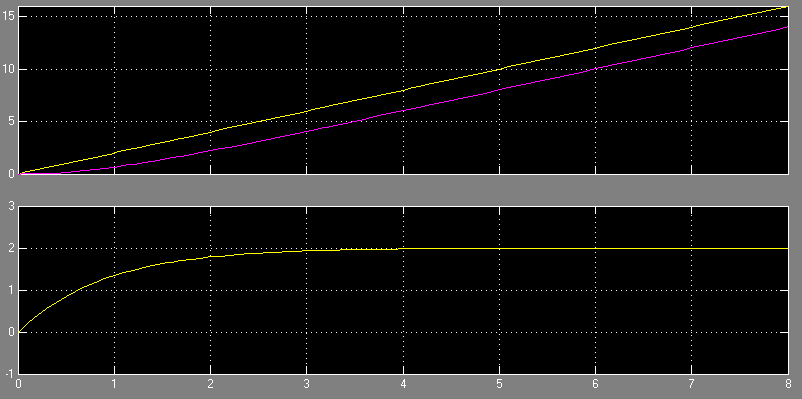
\includegraphics[scale=0.5]{ev.png}
	\captionof{figure}{\textit{Tracés de l'entrée $ e(t) $ en jaune, de la sortie  $ s(t) $ en mauve et celui de l'erreur $\epsilon(t) $. \\}}
	\label{fig2} 
	\end{center} 
	

	\paragraph{} L'erreur de traînage correspond bien à $e_1$ qui vaut $2$ dans notre cas, comme le montre la théorie:\\
	$ \epsilon_v = \underset{p\rightarrow 0}{lim} p \epsilon(p) = \underset{p\rightarrow 0}{lim} p E(p)S(p)  $\\[0.25 cm] 
	Avec : $S(p) = \frac{1}{G(p)+1} =  \frac{p(1+TP)}{p(1+TP)+K_G}$ et $E(p) = \frac{e_1}{p^2}$\\[0.25cm]
	
	$\Rightarrow \epsilon_v = \underset{p\rightarrow 0}{lim}\frac{e_1(1+TP)}{p(1+TP)+K_G}$\\[0.25cm]
	   
	$\Rightarrow \epsilon_v = \frac{e_1}{K_G}=e_1$	   
	   
\section{\textsc{Caractérisation de la réponse fréquentielle}}

	\paragraph{} La réponse fréquentielle est un passe bas comme le montre le tracé de Bode suivant : 
	
	\begin{center}
	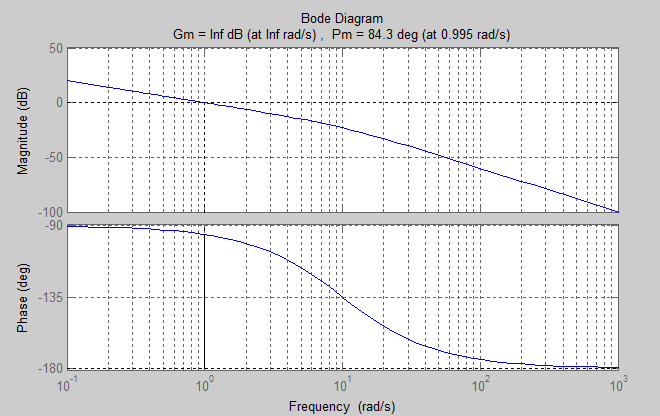
\includegraphics[scale=0.5]{bode1.png}
	\captionof{figure}{\textit{Tracé de Bode en Boucle Ouverte\\}}
	\label{fig3} 
	\end{center}
	
	\par La pulsation de bande passante vaut $1 rad/s.$ \\ 
	
\section{\textsc{Les performances}}
\subsection{\textsc{Stabilité}}

	\par Le système en boucle ouverte donne une marge de gain $MG\rightarrow \infty$ et une marge de phase $MP=84.3>0$, cela assure la stabilité du système. 

\subsection{\textsc{Précision et Rapidité}}

	\par Le système est de type 1 donc l'erreur statique est nulle, le temps de réponse à un échelon unité vaut $t_r=2.78 s.$

	\begin{center}
	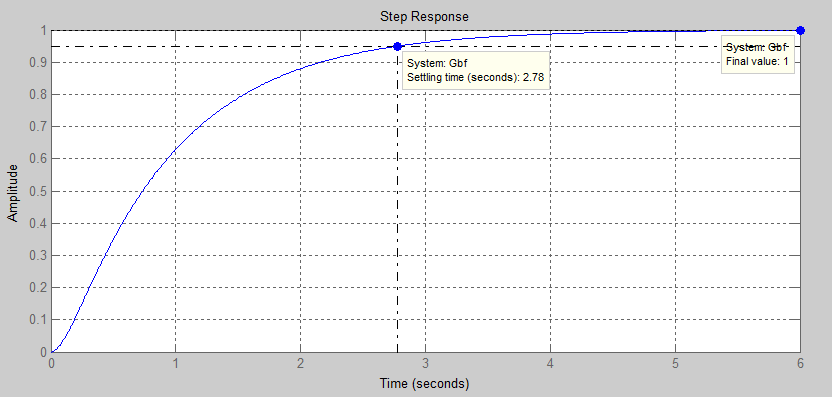
\includegraphics[scale=0.5]{step1.png}
	\captionof{figure}{\textit{Réponse indicielle de la boucle fermée\\}}
	\label{fig4} 
	\end{center}
	